\chapter{Kommunikationsmodel}

\begin{comment}
Im Kommunikationsmodell muss ersichtlich sein, welche Informationen zwischen Nutzern in verschiedenen Rollen über das System ausgetauscht werden sollen. Dabei kann es auch wichtig sein die Reihenfolge der Kommunikationsvorgänge zu spezifizieren. 
\end{comment}

\section{Akteure}

\subsection*{Verwaltungsserver}
\begin{itemize}
\item übergibt Rohdaten und Regeln an Regel-Engine
\item gibt Informationen zum Systemzustand an Steuerungsclient
\item erhält Priorisierungsinformation von Steuerungsclient
\item übergibt priorisiertes Geschäftsobjekt an Verwaltungsclient
\end{itemize}

\subsection*{Steuerungsclient}
\begin{itemize}
\item erhält Information vom Verwaltsdienst zum Systemzustand %@todo verschieben welche Absender aktuell sind wie lange im System
\item teilt Verwaltungsdienst die Priorisierung mit%@todo an andre stelle: nach Eingangsdatum (FIFO), Absender, ggf Anzahl/Absender
\end{itemize}

\subsection*{Verwaltungsclient}
\begin{itemize}
\item erhält aktuell priorisierte Geschäftsobjekte vom Verwaltungsdienst
\item gibt vollständiges Geschäftsobjekt an Verwaltungsdienst zurück
\item gibt unvollständiges Geschäftsobjekt an Fachclient (über Verwaltungsdienst)
\end{itemize}

\subsection*{Fachclient}
\begin{itemize}
\item erhält unvollständiges Geschäftsobjekt von Verwaltungsclient (über Verwaltungsdienst)
\item gibt vervollständigtes Geschäftsobjekt an Verwaltungsdienst zurück
\end{itemize}

\subsection*{Regel-Engine}
\begin{itemize}
\item erhält Geschäftsobjekt und Regel vom Verwaltungsdienst
\end{itemize}


\section{Kommunikationsdiagramm}

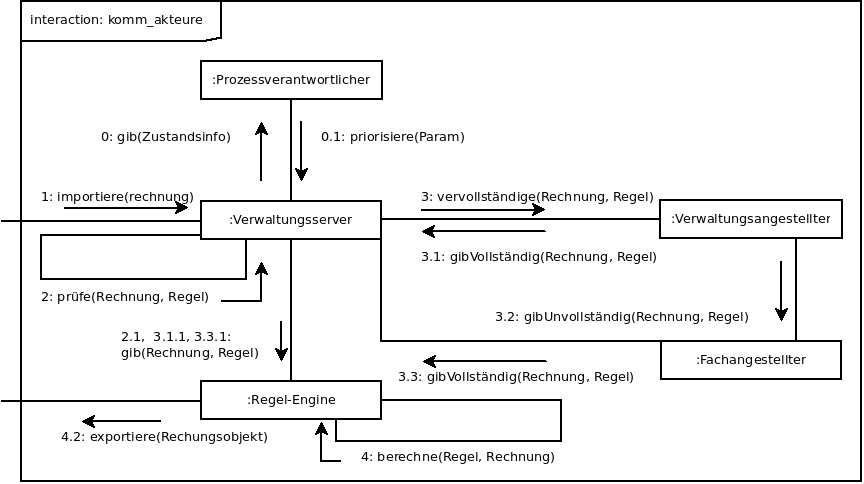
\includegraphics[width=\textwidth]{EISWS1516Howe_Kommunikation.png}
\noindent



